\documentclass[a4paper,10pt]{article}
\usepackage{a4wide}
\usepackage{listings}
\usepackage{mathtools}
\usepackage[english]{babel}
\usepackage{graphicx}
\begin{document}
\section*{Authors, date, assignment}
Authors : Dan Iatco (s2535130) \& Levente Sandor (s2552310)\\
Group: CS 1.Ib.1\\
Date:  26 november 2013\\
Day, Time of the Lab session: Thursday 21 November 2013, 15:00-17:00\\
Autonomous Systems lab 2 "Swarming"\\

\section*{Exercise 1}
Avoid weight: determines how strongly the avoid area is enforced (how fast to avoid a boid)
Align weight: determines how strongly the align area is enforced (how fast to align with a boid)
Center weight: determines how strongly the boids are pulled into the center of their group
Avoid distance: determines the radius of the avoid area
Align distance: determines the radius of the align area
Center distance: determines the radius of the group's center

\section*{Exercise 2}
The boids' spread is not even, because of their environment. The height of the area in which they can
move is smaller than the width of it. Also, if there are too many boids (more than 7), they cannot move
from each other anymore and they get stuck, since their avoid areas are constantly colliding.

\section*{Exercise 3}
For the experiment, we use 40 boids. This number is big enough to demonstrate swarming well, but does not
result in an overcrowded screen. The boids are grouped together with the simulation paused, a target is
selected in a random corner of the area so they have to move the longest way, then the simulation is
started. To consider it a success, more than 50\% of the boids must reach the target (majority). We 
execute 10 repetitions for each different percentage, which should give us a realiable plot.\\
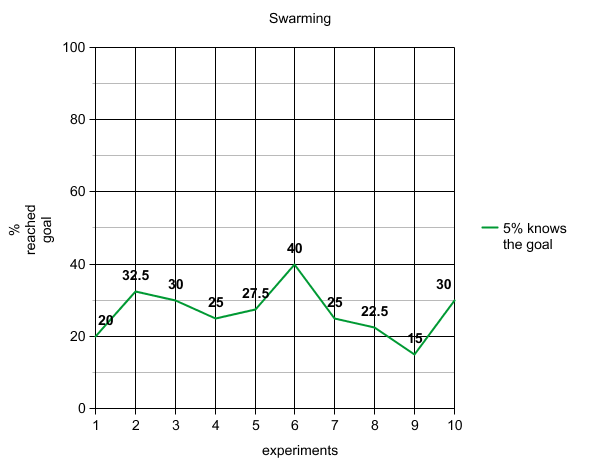
\includegraphics[width=10cm]{graph.png}\\
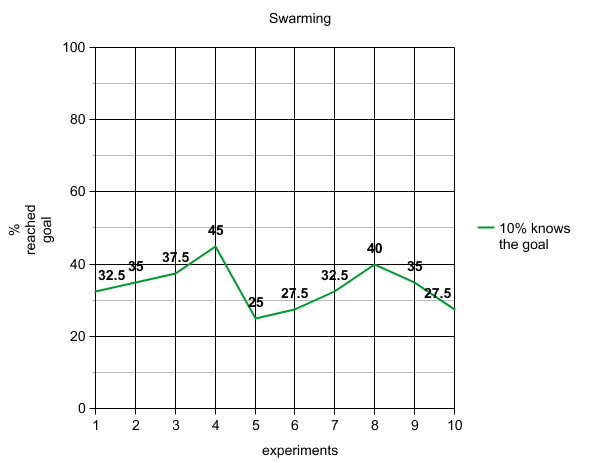
\includegraphics[width=10cm]{graph_1.png}\\
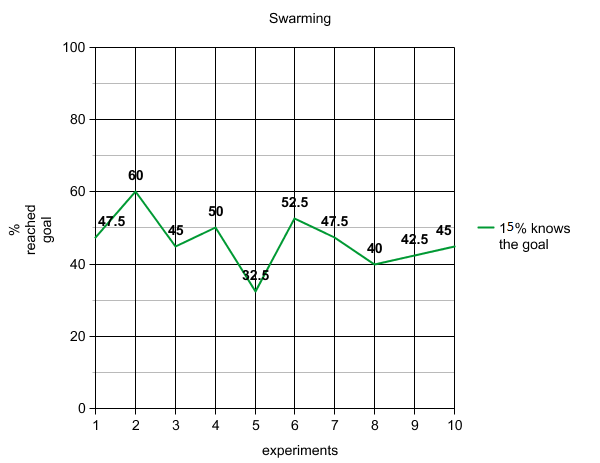
\includegraphics[width=10cm]{graph_2.png}\\
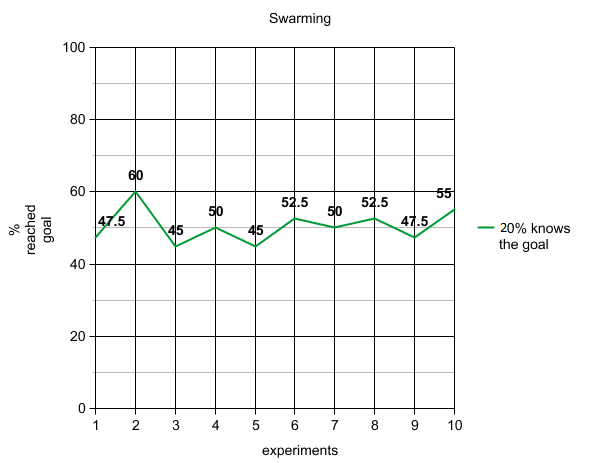
\includegraphics[width=10cm]{graph_3.png}\\
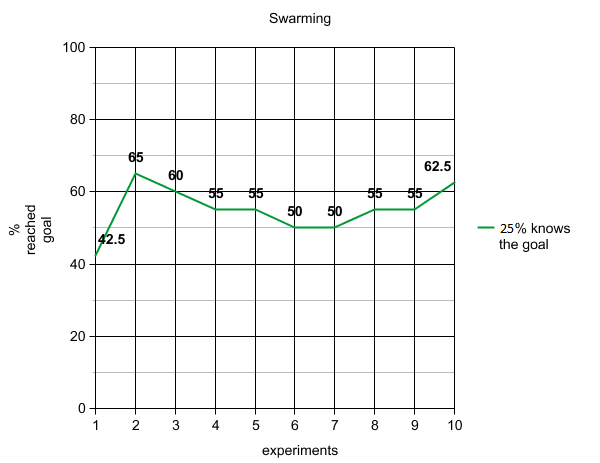
\includegraphics[width=10cm]{graph_4.png}\\
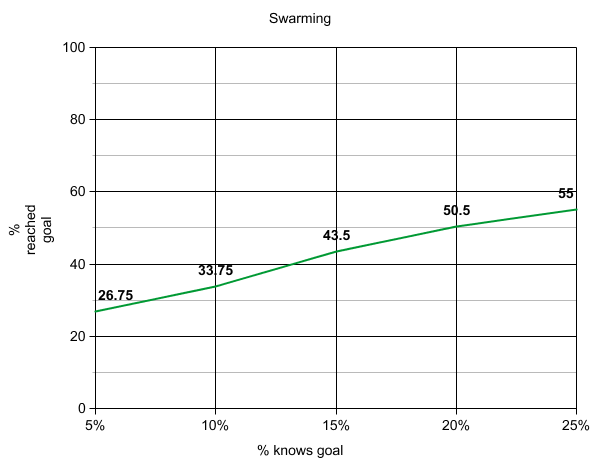
\includegraphics[width=10cm]{ug.png}\\
\end{document}